\documentclass[]{article}
\usepackage{listings} 
\usepackage{algorithm}
\usepackage{algorithmic}
\usepackage{graphicx}
\graphicspath{ {images/} }
\usepackage{float}
\usepackage{geometry}
\usepackage{pdfpages}

%opening
\title{}
\author{}
\date{}
\special{papersize=8.5in,11in}
\geometry{left=1.5cm,right=2cm,top=1.5cm,bottom=1.5cm}

\begin{document}
	
	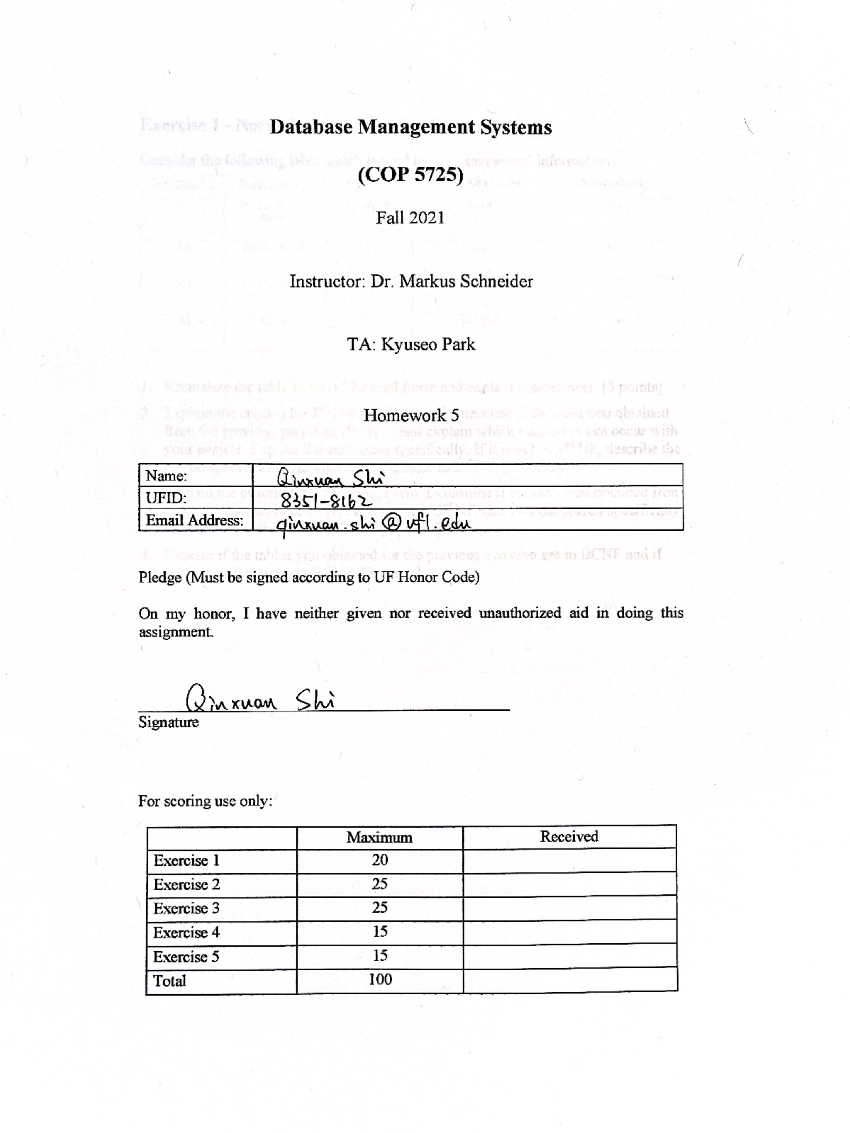
\includepdf{../HWk5.pdf}
	
	\section{Exercise 1}
	
	(1). Normalize the table to the 1st Normal Form and explain your answer. [5 points] \\ 
	
	\noindent Since a relation schema is in first normal form (1NF) if, and only if, the domains of all its attributes only contain atomic (or indivisible) values.   \\
	
	\noindent However, attribute EventNumber and Winning have non-atomic values, which are lists. So the table have to be divided into two tables, A(\underline{CustomerID, EventNumber}, Winning), B(\underline{CustomerID}, customerGrade, DiscountRate). According to the original table, CustomerID and EventNumberthe determine attribute Winning functionally; and only use CustomerID can also determines attributes customerGrade and DiscountRate. As a result, A(\underline{CustomerID, EventNumber}, Winning), B(\underline{CustomerID}, customerGrade, DiscountRate) these two tables are both in 1NF.  \\
	
	\noindent (2). Explain the criteria for 2nd Normal Form and determine if the table you obtained from the previous part is in 2nd NF. Then explain which anomalies can occur with your answer. Explain the anomalies specifically. If it is not in 2nd NF, describe the reason specifically and normalize the table to 2nd NF. [5 points]  \\
	
	\noindent A relation schema R is in the second normal form (2NF) with respect to a set F of FDs if, and only if, it is in 1NF and every nonprime attribute A in R is fully functionally dependent on every candidate key of R.   \\
	
	\noindent Since the 2NF holds automatically for relation schemas with only single-attribute keys, so B(\underline{CustomerID}, customerGrade, DiscountRate) must in 2NF. We only need to consider A(\underline{CustomerID, EventNumber}, Winning). It's easy to find out that the FD (CustomerID, EventNumber$\rightarrow$\ Winning) holds, and (EventNumber$\rightarrow$CustomerID) holds. There is no other FDs and both these FDs are not violeting 2NF. As a result, both A and B are in 2NF.   \\
	
	\noindent There should be anomalies occur in B. Since there are nonprime attributes functionally dependent on other nonprime attributes, (customerGrade$\rightarrow$DiscountRate) and (DiscountRate$\rightarrow$customerGrade).   \\
	
	\noindent (3). Explain the criteria for 3rd Normal Form. Determine if the table you obtained from the previous part is in 3rd NF. If it is not in 3rd NF, describe the reason specifically and normalize the table to 3rd NF. [5 points]  \\
	
	\noindent A relation schema R is in the third normal form (3NF) with respect to a set F of FDs if, and only if, for each FD X → Y in F+ with X → R and Y → R at least one of the following conditions holds: \\
	
	X → Y is a trivial FD \\
	
	X is a superkey of R \\
	
	Every element of Y – X is a prime attribute of R \\
	
	\noindent To A(\underline{CustomerID, EventNumber}, Winning), (CustomerID, EventNumber) is the primary key, and we could find the FDs F = \{(CustomerID, EventNumber$\rightarrow$Winning), (EventNumber$\rightarrow$CustomerID)\}. It's easy to find that $F^{+}$ will only add trivial FDs to F, they all hold for 3NF, so we only need to consider these two FDs. \\
	
	\noindent To the first FD (CustomerID, EventNumber)$\rightarrow$Winning, since {CustomerID, EventNumber} is the primary key, so it holds.  \\
	
	\noindent To the second FD EventNumber$\rightarrow$CustomerID, it is not trivial, and also not superkey. CustomerID - EventNumber = CustomerID $\in$prime attributes.   \\
	
	\noindent To B(\underline{CustomerID}, customerGrade, DiscountRate), CustomerID is primary key, and the FDs F = \{(CustomerId$\rightarrow$customerGrade, DiscountRate), customerGrade$\rightarrow$DiscountRate, DiscountRate$\rightarrow$customerGrade\}. There is no other FDs except trivial FDs.   \\
	
	\noindent Follow the same steps as A, customerGrade$\rightarrow$DiscountRate, DiscountRate$\rightarrow$customerGrade violates 3NF. So B is not in 3NF.   \\ 
	
	\noindent Normalize B to 3NF. (CustomerId as C, customerGrade as G, DiscountRate as D) \\
	
	\noindent Step1: minimal cover of F = \{C$\rightarrow$G, G$\rightarrow$D, D$\rightarrow$G\}  \\
	
	f1 = C$\rightarrow$G,\\
	
	f2 = G$\rightarrow$D,\\
	
	f3 = D$\rightarrow$G \\
	
	\noindent Step2: Generation of relation schemas from the FDs  \\
	
	R1 = \{C, G\}, F1 = f1 \\
	
	R2 = \{G, D\}, F2 = f2, f3 \\
	
	R3 = \{D, G\}, F3 = f2, f3 \\
	
	\noindent Step3: the candidate key C contained in R1.  \\
	
	\noindent Step4: R3$\sqsubseteq$R2  \\
	
	\noindent Step5: \{(R1, F1), (R2, F2)\} = \\
	
	\{
		(\{\underline{CustomerId}, customerGrade\}, \{CustomerId$\rightarrow$customerGrade\}), 
		(\{\underline{customerGrade}, DiscountRate\}, \{DiscountRate$\rightarrow$customerGrade, customerGrade$\rightarrow$DiscountRate\})
	\}
	
	\noindent As a result, A is in 3NF. B is normalized into C(CustomerId, customerGrade) and D(customerGrade, DiscountRate). \\
	
	\noindent (4). Explain if the tables you obtained for the previous question are in BCNF and if not, normalize them to BCNF. [5 points] \\
	
	\noindent To A(\underline{CustomerID, EventNumber}, Winning), \{(CustomerID, EventNumber$\rightarrow$Winning), (EventNumber$\rightarrow$CustomerID)\} is in BCNF.  \\
	
	\noindent To C(CustomerId, customerGrade), \{CustomerId$\rightarrow$customerGrade\} is in BCNF. \\
	
	\noindent To D(customerGrade, DiscountRate), \{DiscountRate$\rightarrow$customerGrade, customerGrade$\rightarrow$DiscountRate\} is also in BCNF. \\
	
	\noindent As a result, A(\underline{CustomerID, EventNumber}, Winning), C(CustomerId, customerGrade) and D(customerGrade, DiscountRate), all these tables are in BCNF.  \\
	
	\section{Exercise 2}
	
	Consider the relation schema R = (A, B, C, D, E) for the following questions.  \\
	
	\noindent 1. Assume we have the following functional dependencies: AB → C, D → A, C → E. Briefly explain if the relation R is in 2NF? If not, what modifications can be made to normalize it into 2NF. [5 points]   \\
	
	\noindent The relation R is not in 2NF, since according to the FDs, the candidate key is BD. However, BD$\rightarrow$A is not left-reduced since D$\rightarrow$A, which violates 2NF.  \\
	
	\noindent Decompose the relation schema R into R1(\underline{B, D}, C, E) and R2(\underline{D}, A). Both two schemas are in 2NF. \\
	
	\noindent 2. Is R in 2NF with the following functional dependencies? If not, normalize it. [5 points]   \\
	
	\noindent AB → D, C → E, E → C, C → A, A → C  \\
	
	\noindent According to the FDs, the candidate keys are BC and BE. Non-prime attributes are A, D. We can know that BC$\rightarrow$D is fully dependent since (C → A, AB → D) and there is no subset of BC, which is B or C that can determines D. It is the same as BE$\rightarrow$D. However, BC$\rightarrow$A violates 2NF, because C$\rightarrow$A; and to BE$\rightarrow$A, E$\rightarrow$A also violates 2NF.  \\
	
	\noindent Decompose the relation schema R into R1(\underline{A, B}, D) and R2(\underline{C}, A, E). Both two schemas are in 2NF. \\
	
	\noindent 3. Are the relations from the answer to question 2 in 3NF? If not, normalize them. [5 points]   \\
	
	\noindent To R1(\underline{A, B}, D), we have FDs F = \{AB → D\}, AB is candidate key, so R1 is in 3NF.  \\
	
	\noindent To R2(\underline{C}, A, E), we have FDs F = \{C → E, E → C, C → A, A → C\}, C is candidate key. However, according to the transitivity rules, E → A and A → E holds, which violates 3NF. \\
	
	\noindent Normalize R2(\underline{C}, A, E).  \\
	
	\noindent Step1: minimal cover of F = \{C → E, E → C, C → A, A → C\}  \\
	
	f1 = C$\rightarrow$E,\\
	
	f2 = E$\rightarrow$C,\\
	
	f3 = C$\rightarrow$A, \\
	
	f4 = A$\rightarrow$C  \\
	
	\noindent Step2: Generation of relation schemas from the FDs  \\
	
	R1 = \{C, E\}, F1 = f1, f2 \\
	
	R2 = \{E, C\}, F2 = f2, f1 \\
	
	R3 = \{C, A\}, F3 = f3, f4 \\
	
	R4 = \{A, C\}, F4 = f4, f3 \\
	
	\noindent Step3: the candidate key C contained in R1, R2, R3, R4.  \\
	
	\noindent Step4: R2$\sqsubseteq$R1, R4$\sqsubseteq$R3  \\
	
	\noindent Step5: \{(R1, F1), (R2, F2)\} = \\
	
	\{
	(\{C, E\}, \{C → E, E → C\}), 
	(\{C, A\}, \{C → A, A → C\})
	\}  \\
	
	\noindent As a result, the relation R is decomposed into R1(\underline{A, B}, D), R2(\underline{C, E}) and R3(\underline{C, A}).   \\
	
	\noindent 4. Are the relations from the answer to question 3 in BCNF? If not, identify FDs that violate BCNF and normalize them. [5 points].   \\
	
	\noindent To R1(\underline{A, B}, D), F=\{AB → D\}, AB is super key, so R1 is in BCNF. \\
	
	\noindent To R2(\underline{C, E}), F=\{C → E, E → C\}, both $C^{+}$ and $E^{+}$ are equal to R2, so R2 is in BCNF.  \\
	
	\noindent To R3(\underline{C, A}), F=\{C → A, A → C\}, both $C^{+}$ and $A^{+}$ are equal to R3, so R3 is in BCNF.  \\
	
	\noindent As a result, all schemas R1(\underline{A, B}, D), R2(\underline{C, E}) and R3(\underline{C, A}) are in BCNF.  \\
	
	\noindent 5. Assume we have the following functional dependencies in F: \{A → B, B → C, A → C, C → A\}. We decompose R(A,B,C) into schemas R1(A, B) and R2(A, C). Show whether it is dependency preserving by using one of the algorithms that covered in the lecture. [5 points]   \\
	
	\noindent Step 1: Compute the closure of F  \\
	
	power set of R=\{$\emptyset$, A, B, C, AB, AC, BC, ABC\} \\
	
	$A^{+}$: ABC  \\
	
	$\Longrightarrow$ $A\rightarrow A, A\rightarrow B, A\rightarrow C, A\rightarrow AB, A\rightarrow AC, A\rightarrow BC, A\rightarrow ABC$ (7FDs)  \\
	
	$B^{+}$: ABC  \\
	
	$\Longrightarrow$ $B\rightarrow A, B\rightarrow B, B\rightarrow C, B\rightarrow AB, B\rightarrow AC, B\rightarrow BC, B\rightarrow ABC$ (7FDs)  \\
	
	$C^{+}$: ABC  \\
	
	$\Longrightarrow$ $C\rightarrow A, C\rightarrow B, C\rightarrow C, C\rightarrow AB, C\rightarrow AC, C\rightarrow BC, C\rightarrow ABC$ (7FDs)  \\
	
	$AB^{+}$: ABC  \\
	
	$\Longrightarrow$ $AB\rightarrow A, AB\rightarrow B, AB\rightarrow C, AB\rightarrow AB, AB\rightarrow AC, AB\rightarrow BC, AB\rightarrow ABC$ (7FDs)  \\
	
	$AC^{+}$: ABC  \\
	
	$\Longrightarrow$ $AC\rightarrow A, AC\rightarrow B, AC\rightarrow C, AC\rightarrow AB, AC\rightarrow AC, AC\rightarrow BC, AC\rightarrow ABC$ (7FDs)  \\
	
	$BC^{+}$: ABC  \\
	
	$\Longrightarrow$ $BC\rightarrow A, BC\rightarrow B, BC\rightarrow C, BC\rightarrow AB, BC\rightarrow AC, BC\rightarrow BC, BC\rightarrow ABC$ (7FDs)  \\
	
	$ABC^{+}$: ABC  \\
	
	$\Longrightarrow$ $ABC\rightarrow A, ABC\rightarrow B, ABC\rightarrow C, ABC\rightarrow AB, ABC\rightarrow AC, ABC\rightarrow BC, ABC\rightarrow ABC$ (7FDs)  \\
	
	\noindent Step 2: Compute the restrictions of F+ to the Ri   \\
	
	$F_{R1} = \{A\rightarrow A, B\rightarrow B, A\rightarrow B, B\rightarrow A, A\rightarrow AB, B\rightarrow AB, AB\rightarrow A, AB\rightarrow B, AB\rightarrow AB\}$ and $F_{R2} = \{A\rightarrow A, C\rightarrow C, A\rightarrow C, C\rightarrow A, A\rightarrow AC, C\rightarrow AC, AC\rightarrow A, AC\rightarrow C, AC\rightarrow AC\}$  \\
	
	\noindent Step 3: Form the union of all restrictions   \\
	
	$F_{r} = \{A\rightarrow A, B\rightarrow B, A\rightarrow B, B\rightarrow A, A\rightarrow AB, B\rightarrow AB, AB\rightarrow A, AB\rightarrow B, AB\rightarrow AB, C\rightarrow C, A\rightarrow C, C\rightarrow A, A\rightarrow AC, C\rightarrow AC, AC\rightarrow A, AC\rightarrow C, AC\rightarrow AC\}$  \\
	
	\noindent Step 4: Compute the closure of Fr   \\
	
	It's easy to know that $F_{r}^{+}$ is just like the $F^{+}$ \\

	\noindent Step 5: Check if the two closures are equal   \\
	
	Two closures are equal, so the decompose is dependency preserving.  \\
	
	\section{Exercise 3}
	
	1. For the relation schema R = (A,B,C,D,E,F,G) and functional dependencies F = \{AB → C, C → A, BC → D, ACD → B, D → EG, BE → C, CG → BD, CE → G\}, determine whether the following decomposition is lossless. Also, determine if it is dependency preserving.  \\
	
	\noindent P = \{R1(AB), R2(BC), R3(ABE), R4(DEF)\} [10 points]  \\
	
	\begin{table}[H]
		\begin{tabular}{|l|l|l|l|l|l|l|}
			\hline
			A & B & C  & D  & E  & F  & G  \\ \hline
			a & b & c1 & d1 & e1 & f1 & g1 \\ \hline
			a2 & b & c & d2 & e2 & f2 & g2 \\ \hline
			a & b & c3 & d3 & e & f3 & g3 \\ \hline
			a4 & b4 & c4 & d & e & f & g4 \\ \hline
		\end{tabular}
	\end{table}

	AB$\rightarrow$C  \\
	
	\begin{table}[H]
		\begin{tabular}{|l|l|l|l|l|l|l|}
			\hline
			A & B & C  & D  & E  & F  & G  \\ \hline
			a & b & c1 & d1 & e1 & f1 & g1 \\ \hline
			a2 & b & c & d2 & e2 & f2 & g2 \\ \hline
			a & b & c1 & d3 & e & f3 & g3 \\ \hline
			a4 & b4 & c4 & d & e & f & g4 \\ \hline
		\end{tabular}
	\end{table}

	C$\rightarrow$A   \\
	
	\begin{table}[H]
		\begin{tabular}{|l|l|l|l|l|l|l|}
			\hline
			A & B & C  & D  & E  & F  & G  \\ \hline
			a & b & c1 & d1 & e1 & f1 & g1 \\ \hline
			a2 & b & c & d2 & e2 & f2 & g2 \\ \hline
			a & b & c1 & d3 & e & f3 & g3 \\ \hline
			a4 & b4 & c4 & d & e & f & g4 \\ \hline
		\end{tabular}
	\end{table}

	BC$\rightarrow$D   \\
	
	\begin{table}[H]
		\begin{tabular}{|l|l|l|l|l|l|l|}
			\hline
			A & B & C  & D  & E  & F  & G  \\ \hline
			a & b & c1 & d1 & e1 & f1 & g1 \\ \hline
			a2 & b & c & d2 & e2 & f2 & g2 \\ \hline
			a & b & c1 & d1 & e & f3 & g3 \\ \hline
			a4 & b4 & c4 & d & e & f & g4 \\ \hline
		\end{tabular}
	\end{table}

	ACD$\rightarrow$B   \\
	
	\begin{table}[H]
		\begin{tabular}{|l|l|l|l|l|l|l|}
			\hline
			A & B & C  & D  & E  & F  & G  \\ \hline
			a & b & c1 & d1 & e1 & f1 & g1 \\ \hline
			a2 & b & c & d2 & e2 & f2 & g2 \\ \hline
			a & b & c1 & d1 & e & f3 & g3 \\ \hline
			a4 & b4 & c4 & d & e & f & g4 \\ \hline
		\end{tabular}
	\end{table}

	D$\rightarrow$EG   \\
	
	\begin{table}[H]
		\begin{tabular}{|l|l|l|l|l|l|l|}
			\hline
			A & B & C  & D  & E  & F  & G  \\ \hline
			a & b & c1 & d1 & e & f1 & g3 \\ \hline
			a2 & b & c & d2 & e2 & f2 & g2 \\ \hline
			a & b & c1 & d1 & e & f3 & g3 \\ \hline
			a4 & b4 & c4 & d & e & f & g4 \\ \hline
		\end{tabular}
	\end{table}
	
	BE$\rightarrow$C   \\
	
	\begin{table}[H]
		\begin{tabular}{|l|l|l|l|l|l|l|}
			\hline
			A & B & C  & D  & E  & F  & G  \\ \hline
			a & b & c1 & d1 & e & f1 & g3 \\ \hline
			a2 & b & c & d2 & e2 & f2 & g2 \\ \hline
			a & b & c1 & d1 & e & f3 & g3 \\ \hline
			a4 & b4 & c4 & d & e & f & g4 \\ \hline
		\end{tabular}
	\end{table}

	CG$\rightarrow$BD   \\
	
	\begin{table}[H]
		\begin{tabular}{|l|l|l|l|l|l|l|}
			\hline
			A & B & C  & D  & E  & F  & G  \\ \hline
			a & b & c1 & d1 & e & f1 & g3 \\ \hline
			a2 & b & c & d2 & e2 & f2 & g2 \\ \hline
			a & b & c1 & d1 & e & f3 & g3 \\ \hline
			a4 & b4 & c4 & d & e & f & g4 \\ \hline
		\end{tabular}
	\end{table}

	CE$\rightarrow$G   \\
	
	\begin{table}[H]
		\begin{tabular}{|l|l|l|l|l|l|l|}
			\hline
			A & B & C  & D  & E  & F  & G  \\ \hline
			a & b & c1 & d1 & e & f1 & g3 \\ \hline
			a2 & b & c & d2 & e2 & f2 & g2 \\ \hline
			a & b & c1 & d1 & e & f3 & g3 \\ \hline
			a4 & b4 & c4 & d & e & f & g4 \\ \hline
		\end{tabular}
	\end{table}
	
	\noindent the decomposition is lossy.  \\
	
	\noindent Dependency Preserving:  \\
	
	\noindent F = \{AB → C, C → A, BC → D, ACD → B, D → EG, BE → C, CG → BD, CE → G\}  \\
	
	\noindent P = \{R1(AB), R2(BC), R3(ABE), R4(DEF)\}   \\
	
	AB$\rightarrow$C: result = AB \\
	
	oldresult = AB, C := closure(F, AB$\cap$AB)$\cap$AB = AB, result = AB; C := closure(F, AB$\cap$BC)$\cap$BC = B, result = AB; C := closure(F, AB$\cap$ABE)$\cap$ABE = ABE, result = ABE; C := closure(F, ABE$\cap$DEF)$\cap$DEF = E, result = ABE;   \\
	
	oldresult = ABE, C := closure(F, ABE$\cap$AB)$\cap$AB = AB, result = ABE; C := closure(F, ABE$\cap$BC)$\cap$BC = B, result = ABE; C := closure(F, ABE$\cap$ABE)$\cap$ABE = ABE, result = ABE; C := closure(F, ABE$\cap$DEF)$\cap$DEF = E, result = ABE;   \\
	
	oldresult = result, C$\cap$ABE is $\emptyset$, so it is not dependency preserving.   \\
	
	\noindent 2. Consider the relation schema R = (A,B,C,D,E).  \\
	
	\noindent a. For functional dependencies F = \{AB → C, BC → D, AD → E\}, is P = \{R1(ABC), R2(BCD), R3(ADE)\} a lossless decomposition? Show all the steps.  \\
	
	\begin{table}[H]
		\begin{tabular}{|l|l|l|l|l|}
			\hline
			A & B & C & D  & E  \\ \hline
			a & b & c & d1 & e1 \\ \hline
			a2 & b & c & d & e2 \\ \hline
			a & b3 & c3 & d & e \\ \hline
		\end{tabular}
	\end{table}

	AB$\rightarrow$C \\
	
	\begin{table}[H]
		\begin{tabular}{|l|l|l|l|l|}
			\hline
			A & B & C & D  & E  \\ \hline
			a & b & c & d1 & e1 \\ \hline
			a2 & b & c & d & e2 \\ \hline
			a & b3 & c3 & d & e \\ \hline
		\end{tabular}
	\end{table}
	
	BC$\rightarrow$D \\
	
	\begin{table}[H]
		\begin{tabular}{|l|l|l|l|l|}
			\hline
			A & B & C & D  & E  \\ \hline
			a & b & c & d & e1 \\ \hline
			a2 & b & c & d & e2 \\ \hline
			a & b3 & c3 & d & e \\ \hline
		\end{tabular}
	\end{table}

	AD$\rightarrow$E \\
	
	\begin{table}[H]
		\begin{tabular}{|l|l|l|l|l|}
			\hline
			A & B & C & D  & E  \\ \hline
			a & b & c & d & e \\ \hline
			a2 & b & c & d & e2 \\ \hline
			a & b3 & c3 & d & e \\ \hline
		\end{tabular}
	\end{table}
	
	\noindent The first row becomes to t, so P is a lossless decomposition.  \\
	
	\noindent b. For functional dependencies F = \{A → CD, B → CE, E → B\}, give a lossless-join decomposition of R into BCNF.  \\
	
	\noindent Since all FDs do not have a left-hand side which is super key, R is not in BCNF. \\
	
	\noindent A → CD is the first FD that violates BCNF, we can get $A^{+}=ACD$, so we decompose R into R1(A, C, D) and R2(A, B, E). Add R1 and R2 to D.  \\ 
	
	\noindent To compute F1, Fs=$\emptyset$, R1=\{A, C, D\}   \\
	
	A$\sqsubseteq$R1, $A^{+}=ACD$, Fs = \{A$\rightarrow$CD\};   \\
	
	C$\sqsubseteq$R1, $C^{+}=C$, Fs = \{A$\rightarrow$CD\};   \\
	
	D$\sqsubseteq$R1, $D^{+}=D$, Fs = \{A$\rightarrow$CD\};   \\
	
	\noindent F1 = \{A$\rightarrow$CD\}   \\
	
	\noindent we can know that R1 is in BCNF.  \\
	
	\noindent To compute F2, Fs=$\emptyset$, R2=\{A, B, E\}   \\
	
	A$\sqsubseteq$R2, $A^{+}=A$, Fs = \{$\emptyset$\};   \\
	
	B$\sqsubseteq$R2, $B^{+}=BE$, Fs = \{B$\rightarrow$E\};   \\
	
	E$\sqsubseteq$R2, $E^{+}=BE$, Fs = \{B$\rightarrow$E, E$\rightarrow$B\};   \\
	
	\noindent F2 = \{B$\rightarrow$E, E$\rightarrow$B\}   \\
	
	\noindent However, R2 is still not in BCNF. We find that B$\rightarrow$E is the first FD that violates BCNF, $B^{+}=BE$, R2 is decomposed into R21(B, E) and R22(A, B).   \\
	
	\noindent To compute F21, Fs=$\emptyset$, R21=\{B, E\}, F2 = \{B$\rightarrow$E, E$\rightarrow$B\}   \\
	
	B$\sqsubseteq$R21, $B^{+}=BE$, Fs = \{B$\rightarrow$E\};   \\
	
	E$\sqsubseteq$R21, $E^{+}=BE$, Fs = \{B$\rightarrow$E, E$\rightarrow$B\};   \\

	\noindent F21 = \{B$\rightarrow$E, E$\rightarrow$B\}   \\
	
	\noindent we can also know that R21 is in BCNF.  \\
	
	\noindent To compute F22, Fs=$\emptyset$, R22=\{A, B\}   \\
	
	A$\sqsubseteq$R22, $A^{+}=A$, Fs = \{$\emptyset$\};   \\
	
	B$\sqsubseteq$R22, $B^{+}=B$, Fs = \{$\emptyset$\};   \\
	
	\noindent F22 = \{$\emptyset$\}   \\
	
	\noindent As a result, R is decomposed into R1(A, C, D), R21(B, E) and R22(A, B), F1 = \{A$\rightarrow$CD\}, F21 = \{B$\rightarrow$E, E$\rightarrow$B\} and F22 = \{$\emptyset$\}. All these schemas are in BCNF.  \\
	
	\noindent c. For functional dependencies F = \{A → CD, B → CE, E → B\}, give a lossless-join decomposition of R into 3NF preserving functional dependencies.  \\
	
	\noindent Minimal Cover of $F_{c}$:=  \{A → CD, B → CE, E → B\} \\
	
	\noindent Step1: minimal cover of F = $F_{c}$  \\
	
	f1 = A → CD,\\
	
	f2 = B → CE,\\
	
	f3 = E → B, \\
	
	\noindent Step2: Generation of relation schemas from the FDs  \\
	
	R1 = \{A, C, D\}, F1 = f1 \\
	
	R2 = \{B, C, E\}, F2 = f2, f3 \\
	
	R3 = \{B, E\}, F3 = f3 \\
	
	\noindent Step3: the candidate keys AB and AE are not contained in R1, R2, R3. So add R4(A, B) to the schemas. \\
	
	\noindent Step4: R3$\sqsubseteq$R2.  \\
	
	\noindent Step5: \{(R1, F1), (R2, F2), (R3)\} = \\
	
	\{
	(\{A, C, D\}, \{A → CD\}), 
	(\{B, C, E\}, \{B → CE, E → B\}),
	(\{A, B\}, $\emptyset$)
	\}  \\
	
	\section{Exercise 4}
	
	Suppose we have a relation schema R(A, B, C, D, E, F, G) and a set of functional dependencies F = \{B → D, DG → C, BD → E, AG → B, ADG → B, ADG → C\}. Decompose R into 3NF by using the 3NF synthesis algorithm. Show all steps and argue precisely. Is this decomposition also in BCNF? If so, why. If not, why not? [15 points]  \\
	
	\noindent Minimal Cover of $F_{c}$:=  \{B → D, DG → C, B → E, AG → B\} \\
	
	\noindent Step1: minimal cover of F = $F_{c}$  \\
	
	f1 = B → D,\\
	
	f2 = DG → C,\\
	
	f3 = B → E, \\
	
	f4 = AG → B  \\
	
	\noindent Step2: Generation of relation schemas from the FDs  \\
	
	R1 = \{B, D\}, F1 = f1 \\
	
	R2 = \{C, D, G\}, F2 = f2 \\
	
	R3 = \{B, E\}, F3 = f3 \\
	
	R4 = \{A, G, B\}, F4 = f4 \\
	
	\noindent Step3: the candidate key AGF is not contained in R1, R2, R3, R4. So add R5(A, G, F) to the schemas. \\
	
	\noindent Step4: there's no redundant relation schemas.  \\
	
	\noindent Step5: \{(R1, F1), (R2, F2), (R3, F3), (R4, F4), (R5)\} = \\
	
	\{
	(\{B, D\}, \{B → D\}), 
	(\{C, D, G\}, \{DG → C\}),
	(\{B, E\}, \{B → E\}),
	(\{A, G, B\}, \{AG → B\}),
	(\{A, G, F\}, $\emptyset$)
	\}  \\
	
	\noindent this decomposition is also in BCNF. Since to R1, $B^{+} = BD = R1$, which means B is super key. It is the same to R2, R3, R4 and R5, the left-hand FDs are all super key. \\
	
	\section{Exercise 5}
	
	1. Add constraints to the table TAKES that checks STUDENT\_NO and COURSE\_NO refer to columns STUDENT.STNO and COURSE.CRNO, respectively. The constraint should guarantee that once a student or course are deleted from STUDENT or COURSE tables, the corresponding records in TAKES table are also deleted. [3 points]  \\
	
	ALTER TABLE TAKES ADD CONSTRAINT TCS FOREIGN KEY (STUDENT\_NO) REFERENCES STUDENT(STNO)
		on delete cascade;  \\
	
	ALTER TABLE TAKES ADD CONSTRAINT TCC FOREIGN KEY (COURSE\_NO) REFERENCES COURSE(CRNO)
		on delete cascade;  \\
	
	\noindent 2. Create primary constraints for STNO and CRNO on the STUDENT and COURSE tables. Create a constraint that check STUDENT.EMAIL is unique. Create constraints that check TAKES.GRADE is not greater than 4 and COURSE.CREDIT is less than 9. [4 points]   \\
	
	ALTER TABLE STUDENT ADD PRIMARY KEY (STNO);  \\
	
	ALTER TABLE COURSE ADD PRIMARY KEY (CRNO);  \\
	
	ALTER TABLE STUDENT ADD UNIQUE (EMAIL);   \\
	
	ALTER TABLE TAKES ADD CHECK (GRADE $\leq$ 4);   \\
	
	ALTER TABLE COURSE ADD CHECK (CREDIT \textless\  9);   \\
	
	\noindent 3. Create a trigger that displays the average grades of students for course (identified by COURSE\_NO), before inserting a record in TAKES table with the same COURSE\_NO. [4 points]   \\
	
	CREATE trigger display
	
	before insert on TAKES
	
	for each row
	
	begin
	
	select avg(GRADE) from TAKES where COURSE\_NO = :new.COURSE\_NO
	
	end; \\
	
	\noindent 4. Create a trigger that inserts STUDENT\_NO, COURSE\_NO and the current timestamp in the STUDENT\_LOG table after inserting or updating a record in the table TAKES. The ID for the new record in the STUDENT\_LOG table should be the current highest ID + 1. [4 points]   \\
	
	CREATE trigger newRecord
	
	after insert or update on TAKES
	
	for each row
	
	begin
	
	insert into STUDENT\_LOG 
	values((select max(ID)+1 from STUDENT\_LOG), :new.STUDENT\_NO, :new.COURSE\_NO, systimestamp)
	
	end; \\
	
\end{document}